\capitulo{6}{Trabajos relacionados}

A continuación, se comparan aplicaciones de referencia o similares usadas por usuarios para obtener lugares de interés turístico. Al final de la sección se presenta una tabla comparativa de estos trabajos relacionados con \textit{Eco City Tours}.
\section{Aplicaciones móviles planificadoras de rutas turísticas}
\subsection{Tripadvisor}
Tripadvisor~\cite{tripadvisor} permite a los usuarios planificar y organizar sus viajes, con recomendaciones basadas en reseñas y experiencias de otros viajeros. Se puede planificar un viaje personalizado indicando fechas pero prioriza los tours de pago, lo que hace difícil seleccionar rutas saludables gratuitas. Además, los establecimientos pueden promocionarse en la plataforma para mejorar su visibilidad lo que interfiere con la objetividad cuando se busca un lugar a visitar.

\subsection{Wanderlog}
Wanderlog~\cite{wanderlog} es una aplicación para la planificación de viajes que simplifica la creación de itinerarios, permitiendo agregar lugares de interés fácilmente. La aplicación tiene infinidad de funcionalidades. Tiene una versión Pro con asistente IA pagando 5 euros al mes. Gratuitamente se pueden enviar 5 mensajes, pero el \acrshort{llm} no almacena ningún contexto de los mensajes previos como se puede ver la imagen \ref{fig:Wanderlog-ia} donde muestra lugares de  Salamanca, pero en la respuesta siguiente cambia a la ciudad de Nueva York, sin haber sido ésta citada. Además, la respuesta ofrecida podría ser el resultado de un prompting sencillo como se puede ver en el prototipo del cuaderno Jupyter \href{https://github.com/fps1001/TFGII_FPisot/tree/main/project-prototypes/prompting.ipynb}{prompting.ipynb}.
\imagen{Wanderlog-ia}{Chatbot de Wanderlog}{.4}

\subsection{Visit A City}
Visit A City~\cite{visitacity} ofrece itinerarios pre diseñados para destinos turísticos, permitiendo a los usuarios explorar lugares recomendados según su tiempo disponible. Aunque el uso de la aplicación es gratis, las rutas son todas comerciales y por tanto de pago, aunque existen lo que la aplicación llama \textit{planes} que son itinerarios generados por los propios usuarios. Las rutas son generadas por aplicaciones de terceros.

\subsection{Tiqets - Museos y Atracciones}
Tiqets~\cite{tiquets} es una aplicación que permite comprar entradas para museos y atracciones, ofreciendo guías digitales para planificar visitas. Sólo muestra información de museos, la gestión de mapas es fija, no se puede modificar el zoom y para rutas usa una aplicación por defecto del dispositivo en el que se ejecuta.

\begin{table}[h]
	\centering
	\renewcommand{\arraystretch}{1.5} % Controla el espaciado entre las líneas
	\rowcolors{2}{gray!20}{white} % Alterna colores de fondo en las filas
	\resizebox{\textwidth}{!}{ % Ajusta el tamaño de la tabla al ancho de la página
		\begin{tabular}{m{4cm} >{\centering\arraybackslash}m{2cm} >{\centering\arraybackslash}m{2cm} >{\centering\arraybackslash}m{2cm} >{\centering\arraybackslash}m{2cm} >{\centering\arraybackslash}m{2.5cm}} % Ajustamos los anchos de las columnas
			\toprule  
			\textbf{Característica} & \textbf{Tripadvisor} & \textbf{Wanderlog} & \textbf{Visit \newline A City} & \textbf{Tiquets} & \textbf{\textit{Eco City Tour}} \\
			\midrule
			Versión de pago & Sí & Sí & No & No & No\\
			Recomendaciones tienen en cuenta factores de sostenibilidad & No & No & No & No & Sí\\
			Modificación dinámica de rutas & Sí & No & No & No & Sí\\
			Intereses de terceros pueden afectar a los resultados & Sí & Sí & No & No & No \\
			Fuente de datos & Propia & Usuarios - LLM & Usuarios & Propia & LLM\\
			Guardado de rutas & Sí & No & Sí & No & Sí\\
			Seguimiento en vivo del usuario & No & No & No & No & Sí \\
			\bottomrule
		\end{tabular}
	}
	\caption{Comparación de aplicaciones}
	\label{herramientasportipodeuso}
\end{table}

\begin{table}[h!]
	\centering
	\renewcommand{\arraystretch}{1.5} % Controla el espaciado entre las líneas
	\begin{tabular}{cc}
	\hline
	\href{https://play.google.com/store/apps/details?id=com.tripadvisor.tripadvisor}{\textbf{Tripadvisor}} & \href{https://play.google.com/store/apps/details?id=com.wanderlog.wanderlog}{\textbf{Wanderlog}} \\
	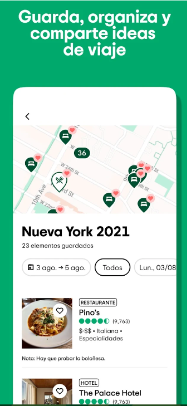
\includegraphics[width=0.32\textwidth]{img/tripadvisor.png} & 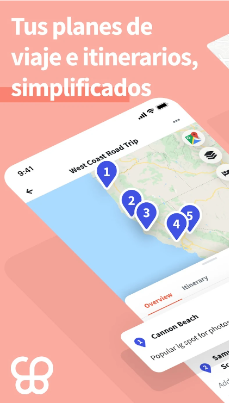
\includegraphics[width=0.34\textwidth]{img/wanderlog.png} \\
	\hline
	\href{https://play.google.com/store/apps/details?id=com.visitacity}{\textbf{Visit A City}} & \href{https://play.google.com/store/apps/details?id=com.tiqets.tiqetsapp}{\textbf{Tiqets - Museos y Atracciones}} \\
	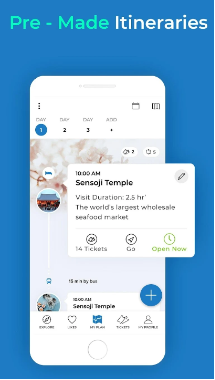
\includegraphics[width=0.35\textwidth]{img/visit_a_city.png} & 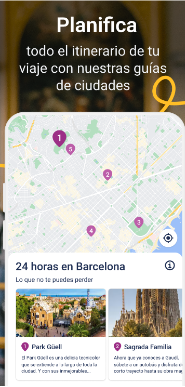
\includegraphics[width=0.31\textwidth]{img/tiquets.png} \\
	\hline
	\end{tabular}
	\caption{Aplicaciones móviles para la planificación de itinerarios turísticos}
	\label{fig:apps_similares}
	\end{table}
	
\section{Otros \acrfull{tfg} }
	\subsection{Chatbot}
	Trabajo Fin de Carrera de José María Redondo Guerra~\cite{chatbot_github} que tuvo como tutores a José Ignacio Santos Martín y Carlos López Nozal.
	
	Este trabajo fue desarrollado usando \acrfull{llm} para la generación de un chat con un sistema \acrshort{rag} para obtener la información de las normas de los \acrshort{tfg} y así mejorar sus respuestas.
	
	\subsection{Visualización de las actividades socioculturales en Castilla y León CULTURALCyL}
	Trabajo Fin de Carrera de Yanela Lozano Pérez con tutores José Ignacio Santos, Virginia Ahedo y Silvia Díaz.
	Esta aplicación mostraba información de eventos culturales para lo cual usaba una aplicación móvil con servicios API.
	Es especialmente interesante como ejemplo de una aplicación móvil con una fuerte característica de usabilidad, ya que se centra en la visualización de mucha información que debe recibir el usuario de manera clara y sencilla.